\subsubsection{Overview}
\label{subsubsec:erlang/overview}

\begin{sloppypar}
The chat server application is implemented by exploiting the supervisor behavior: at startup, the application process spawns a supervisor process (callback module \texttt{chat\_server\_sup}) which will be responsible to manage the lifecycle of the process which runs the \textbf{Cowboy HTTP server}.

The process running Cowboy is implemented as a \textbf{gen\_server} using the module \texttt{cowboy\_listener} as callback module.
The Cowboy server will listen at the port \textbf{8300} waiting for new WebSocket connection requests and it will spawn a new ad hoc process to handle the request once received. Thus, every user will be assigned to a different Erlang process (actually, every user \textit{connection} since a student can open more than one WebSocket connections).


\begin{figure}[ht]
	\centering
	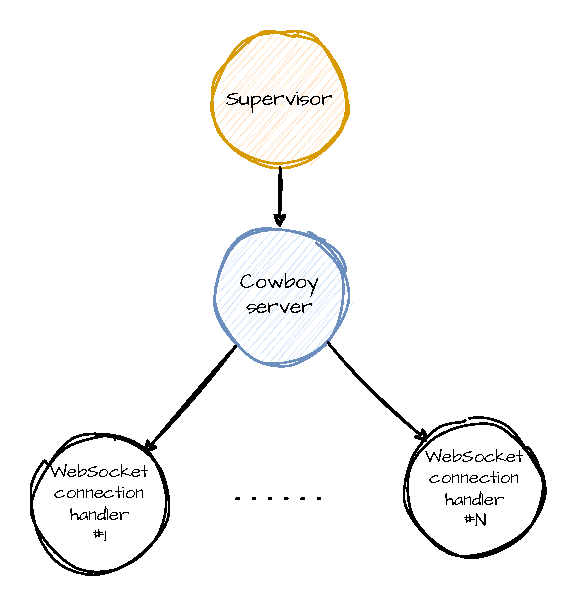
\includegraphics[width=0.5\textwidth]{img/system_architecture/erlang_diagram.pdf}
	\caption{Hierarchy of Erlang processes inside the chat server application}
	\label{fig:erlang-hierarchy}
\end{figure}


The new spawned process will call the functions belonging to the \texttt{chatroom\_websocket} module:
\begin{itemize}
    \item \texttt{init/1}: called whenever a request is received, in order to establish a websocket connection.
    \item \texttt{websocket\_handle/2}: called whenever a text, binary, ping or pong frame arrives from the client. It will handle the reception and deserialization of the JSON objects coming from the client.
    \item \texttt{websocket\_info/2}: called whenever an Erlang message arrives (i.e. a message from another Erlang process). It will forward a chatroom message to the client browser assigned to this process.
    \item \texttt{terminate/3}: called whenever the WebSocket connection is closed. It will remove its assigned user from the list of the currently online students inside the chatroom.
\end{itemize}


\subsubsection{Client-server communication}
\label{subsubsec:erlang/Client-server communication}

During the WebSocket session, all messages exchanged between the \textit{client browser} and the \textit{Cowboy WebSocket handler} are encoded in \textbf{JSON format}. Meanwhile Javascript natively supports JSON encoding/decoding inside the browser, the Erlang application requires an external dependency such as the \href{https://github.com/sile/jsone}{\textbf{jsone library}}.

The client browser can send three different kinds of JSON messages:
\begin{itemize}
    \item Request for login into a chatroom
    \item Request for the list of the currently online students in the chatroom, i.e. the students currently logged in the chatroom
    \item Chat message
\end{itemize}

The Javascript client encodes these message in the following format:
\begin{Verbatim}[samepage=true]
{
    opcode: "LOGIN",
    course: <id of the course owning the chatroom>,
    username: <username of the current user>
}

{
    opcode: "GET_ONLINE_USERS"
}

{
    opcode: "MESSAGE",
    text: <text of message>
}
\end{Verbatim}

On the other hand, the Cowboy server can send back two different kinds of JSON messages:
\begin{itemize}
    \item Current list of the currently online students in the chatroom
    \item Chat message
\end{itemize}

The encoded format is the following:
\begin{Verbatim}[samepage=true]
{
    opcode: "MESSAGE",
    sender: <sender's username>,
    text: <text of message>
}

{
    opcode: "GET_ONLINE_USERS",
    list: <list of currently online users>
}
\end{Verbatim}

\end{sloppypar}


\subsubsection{Modules overview}
The \texttt{chat\_server} application is composed of six modules:
\begin{itemize}
    \item \texttt{chat\_server\_app}: the first executed module. It starts the mnesia application and spawns the supervisor process. It implements the \texttt{application} behavior.
    
    \item \texttt{chat\_server\_sup}: the \texttt{supervisor} callback module. It's responsible to spawn a process which will handle the lifecycle of the process running the Cowboy server. It implements the \texttt{supervisor} behavior.
    
    \item \texttt{cowboy\_listener}: a \texttt{gen\_server} callback module which will start a Cowboy instance listening at port 8300 for TCP connections. It will also cleanup the Mnesia database by removing all the users assigned to this Erlang node which remained after an unexpected crash of the server.
    
    \item \texttt{chatroom\_websocket}: callback module for the module \texttt{cowboy\_websocket}. For more details see section \vref{subsubsec:erlang/overview}.
    \item \texttt{chatroom\_server}: module which implements the business logic for the WebSocket handlers.
    
    \item \texttt{mnesia\_manager}: module which offers methods to access the Mnesia database. For more details see section \vref{subsec:erlang-mnesia}. 
\end{itemize}

